%% ----------------------------------------------------------------------------
% BIWI SA/MA thesis template
%
% Created 09/29/2006 by Andreas Ess
% Extended 13/02/2009 by Jan Lesniak - jlesniak@vision.ee.ethz.ch
%% ----------------------------------------------------------------------------
\newpage
\chapter{Fully annotated segmentation masks}
The deep neural networks have become popular to solve any task in the field of computer vision. To train a network from scratch, the main effort goes into preparing data for training network, and in coming up with best architecture and choosing best training parameters. The data is available on internet and can be extracted and modified for various tasks such as, IMDB database can be used to train network for problem involving faces. This becomes a problem in medical domain where it is very costly to generate images and even more costly and time consuming to prepare it for training. For our problem of image segmentation, we described the problem faced by experts and researchers in generated segmented masks. The lack of data has motivated researchers to use transfer learning. Transfer learning tries to store the knowledge gained from solving one problem and applying it to different but related problem. Thus, in practice, it is very rare to train an entire Convolutional Network from scratch (with random initialization), because it is relatively rare and difficult to have a dataset (images and labels) of sufficient size for training. Instead, it is common to use a pretrained network either to intialize a network or to extract required feature maps. We decided to use pretrained network and fine-tune it for our task.

\section{One shot Video object segmentation (OSVOS)}
Caelles et al[cite] designed an architecture to segment an object in a video sequence using only one frame for training. The network is trained to learn object from only one frame and generate segmentation mask for remaining all frames. The segmentation work well if object remains in relatively similar shape and size. This can be considered similar to our problem of segmenting vesicles in 3D stack of liver tissue. Since, the vesicles are relatively similar in shape and size in different slices, we annotated first few slices to train the network. We generated more data using cropped and flipped slices for training. In literature, we can find that network can overfit on relatively small dataset. The use of augmentation helps in generating more data and avoids network from overfitting. \par
OSVOS uses pretrained network of VGG-net for initialization. They removed the final fully-connected layers and replaced them with deconvolution layers to generate mask of image size. In addition, the network contains end output, side outputs and main output generated from combination of side outputs. The total loss is calculated for all outputs and used for backpropagation. The details of architecture and initialization parameters can be found in Caelles et al[cite]. As we described the diffculty of annotating full objects in Section 1, we tried to observe accuracy improvement with increase of training data. We trained OSVOS from 1 slice and increased the training data to 10 slices. The initialization parameters were kept same for cases. In figure 2.1, we can observe that OSVOS performs well with with only 2 slices. The segmentation output from CNN trained using 2 slices is also shown in figure 2.1.\par
\begin{figure}[h!]\label{fig:cnnslices}
\begin{tabular}{cc}
 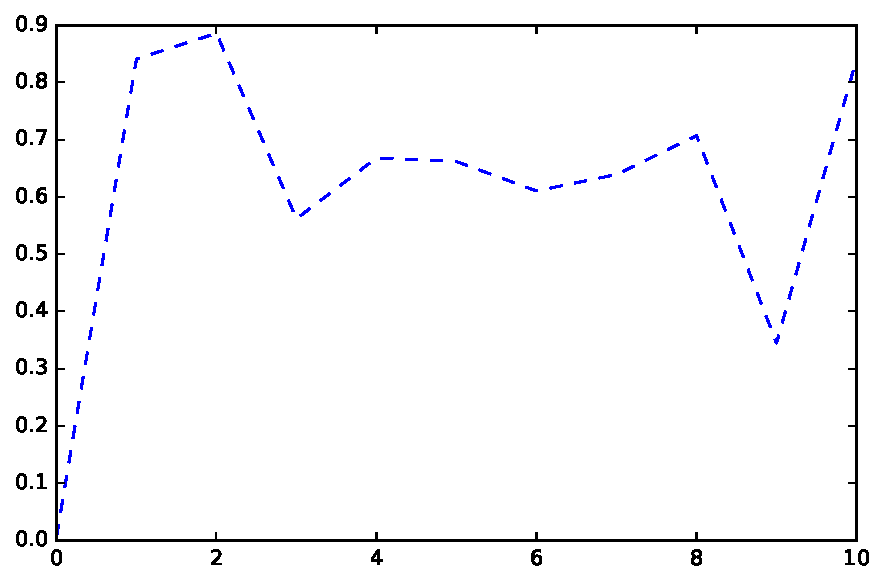
\includegraphics[width=0.5\linewidth]{figures/cnn_diff_slices.pdf} & 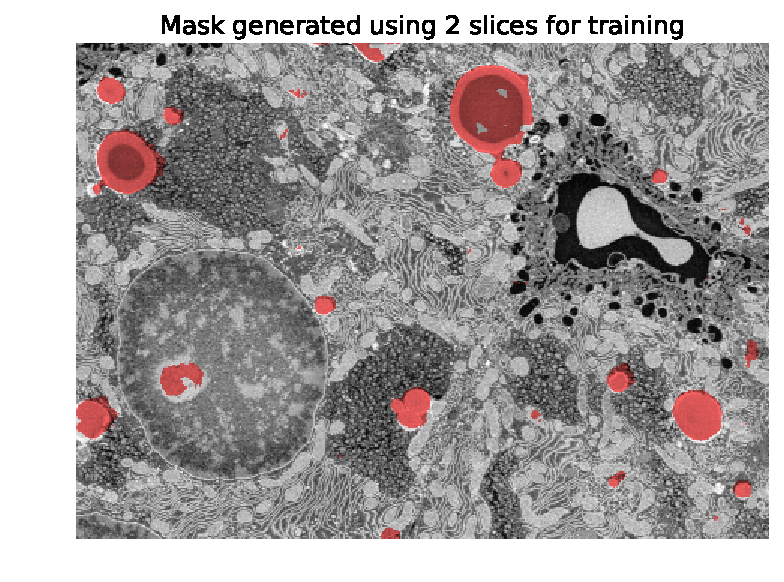
\includegraphics[width=0.5\linewidth]{figures/cnn_mask_2slice.pdf} \\
\end{tabular}
\caption{Left image:- F-measure computed for different amount of training data; Right image: Predicted mask for one slice}
\end{figure}
We expected increase in performance with increase in amount of data. This does not happen as CNN is not able to converge equivalently for all cases. It is important to remember here that annotating one slice is not same as one object. We can observe these multiple objects in figure 1.2. Also, change in annotation will force us to train network again. These difficulties motivated us to try semi-supervised learning for our task of segmentation.
